\documentclass[11pt]{article}
\usepackage{graphicx} % Required for inserting images
\setlength{\parindent}{0pt}
\usepackage[bookmarks=true, colorlinks=true, urlcolor=blue, linkcolor=black]{hyperref}

\usepackage{enumitem}
\usepackage[utf8]{inputenc}
\usepackage[T1]{fontenc}
\usepackage[english]{babel}
\usepackage{geometry}
\usepackage{lastpage}
\usepackage{fancyhdr}
\usepackage{datetime}

% Link to other SOPs, forms
\usepackage{xr}
\externaldocument[101-]{../../100_emergency/1_hardware/sop_101_hardware}
% Definitions for SOP sections 3.
\newcommand{\AdverseEvent}{\textbf{Adverse Event}: Any untoward or unfavorable medical occurrence in a human subject, including any abnormal sign, symptom, or disease, temporally associated with the subject's participation in the research, whether or not considered related to the subject's participation in the research.}

\newcommand{\ControlRoom}{\textbf{Control Room}: B17; The main room of the MRI suite that contains the computer displays and keyboards that control the MRI scanner. The Control Room is accessed from B15 that is controlled by an Electronic Lock.}

\newcommand{\DcmComputer}{\textbf{DICOM Computer}: The Mac Studio located in the Control Room the receives DICOM files from the scanner.}

\newcommand{\ElectronicLock}{\textbf{Electronic Lock}: All doors at the ND-HNC are controlled by electronic locks. The electronic lock system recognizes the owner's Irish1Card, logs the time of the attempted entry, and unlocks the door if the owner has been granted access.}

\newcommand{\EEG}{\textbf{EEG}: Electroencephalograpy, a technique used to measure changes in electromagnetic properties of neural tissue.}

\newcommand{\EquipmentRoom}{\textbf{Equipment Room}: B18; The room containing hardware for MRI operations.}

\newcommand{\FDA}{\textbf{FDA}: Food and Drug Administration.}

\newcommand{\GoodCatch}{\textbf{Good Catch}: Early recognition of an event with the potential to cause damage, injury, or illness.}

\newcommand{\Helper}{\textbf{Helper}: Second person in Zones 3 and 4 who assists in emergency responses, typically Level 2-3.}

\newcommand{\Incident}{\textbf{Incident}: An occurence, action, or event that warrants reporting (e.g. a policy is not followed and/or an individual's health is at risk). Includes Adverse Events, Near Misses, Unanticipated Problems, etc.}

\newcommand{\Lead}{\textbf{Lead}: Primary person in Zones 3 and 4 responsible for the Visitor's safety, in charge during emergency responses. Level 4 operator or MRI Technologist.}

\newcommand{\MagnetRoom}{\textbf{Magnet Room}: B17A; The room within the MRI suite that contains the MRI scanner. It is accessed from within the MRI Control room (B17) through a doorway that is controlled by an Electronic Lock.}

\newcommand{\NearMiss}{\textbf{Near Miss}: An incident that occurred but did not cause personal injury/illness e.g. a small/contained fire, trip on sidewalk or carpeting, falling object.}

\newcommand{\NDHNC}{\textbf{ND-HNC}: Notre Dame Human Neuroimaging Center, Lower Level of Veldman Family Psychology Clinic.}

\newcommand{\Operator}{\textbf{Operator}: MRI Technologist or Level 4 researcher, responsible for conducting research operations and maintaining equpiment. The Lead during emergency responses.}

\newcommand{\PIN}{\textbf{PIN}: Personal Identification Number, separate for Irish1Card and security.}

\newcommand{\ResearchAssistant}{\textbf{Research Assistant}: Individual with access Levels 1-3 to the MRI research suite. Typically the Helper during emergency responses.}

\newcommand{\SeriousInjury}{\textbf{Serious Injury}: An injury or illness that is life threatening; results in permanent impairment of a body function or permanent damage to a body structure; or necessitates medical or surgical intervention to preclude permanent damage or impairment.}

\newcommand{\StimControl}{\textbf{Stimulus Control Computer}: The Windows machines in the Control Room that deploy fMRI tasks and capture participant responses.}

% \newcommand{\Subject}{\textbf{Subject}: An individual who is participating in an experimental protocol at ND-HNC and has not taken the ND-HNC safety course.}

\newcommand{\Supervision}{\textbf{Supervision}: A supervisor is continuously present in both sight and sound range of the individual or task being monitored. This approach ensures the supervisor can actively observe, direct, and immediately intervene if a complication or safety issue arises.}

\newcommand{\TMS}{\textbf{TMS}: Transcranial magnetic stimulation, a technique used to disrupt normal operations of neural tissue.}

\newcommand{\TornadoWarn}{\textbf{Tornado Warning}: A tornado has been sighted or indicated by weather radar and there is imminent danger to life and property. Action is required.}

\newcommand{\TornadoWatch}{\textbf{Tornado Watch}: Tornados are possible in and near the watch area. Be ready to act quickly and move to the designated tornado safe area.}

\newcommand{\UnanticipatedProblem}{\textbf{Unanticipated Problem}: An incident, experience, or outcome that meets \textbf{all} of the following criteria: (1) unexpected (in terms of nature, severity, or frequency) given (a) the research procedures that are described in the protocol-related documents, such as the IRB-approved research protocol and informed consent document; and (b) the characteristics of the subject population being studied; (2) related or possibly related to participation in the research; and (3) suggests that the research places subjects or others at a greater risk of harm than was previously known or recognized.}

\newcommand{\VFPC}{\textbf{VFPC}: Veldman Family Psychology Clinic.}

\newcommand{\Visitor}{\textbf{Visitor}: An individual who has not taken the ND-HNC MRI Safety Course but has a legitimate reason for entering the MRI suites. Research participants and their legal guardians are Visitors. Other Visitors may include: individuals providing/receiving a tour of the VFPC and ND-HNC, faculty and staff who have not received MRI Safety Course, and research assistants.}



% figures and tables
\usepackage{graphicx}
\graphicspath{ {../../pics} }
\usepackage{rotating}
\usepackage{float}
\usepackage{subfig}
\usepackage{caption}
\DeclareCaptionLabelFormat{adja-page}{\hrulefill\\#1 #2 \emph{(previous page)}}


\renewcommand{\headrulewidth}{0pt}
% \newdateformat{yearmonth}{\THEYEAR-\THEMONTH-\THEDAY}
\pagestyle{fancy}
\fancyhead[L]{}
\fancyhead[R]{Approved: TBD}
\fancyfoot[C]{}
\fancyfoot[L]{ND-HNC SOP 302: v.0.2.0}
\fancyfoot[R]{p. \thepage /\pageref*{LastPage}}


% start document
\begin{document}

\renewcommand{\labelenumii}{\arabic{enumi}.\arabic{enumii}}
\renewcommand{\labelenumiii}{\arabic{enumi}.\arabic{enumii}.\arabic{enumiii}}
\renewcommand{\labelenumiv}{\arabic{enumi}.\arabic{enumii}.\arabic{enumiii}.\arabic{enumiv}}

\begin{center}
	\textbf{\Large SOP 302: Fire and Gas Emergencies}\\
	\hrulefill
\end{center}


\section{Summary}
This document establishes  procedures for fire and gas leak emergencies at the Notre Dame Human Neuroimaging Center (ND-HNC), located in the Lower Level of:\\

Veldman Family Psychology Clinic\\
501 North Hill St.\\
South Bend, IN 46617

\section{Scope}
These policies apply to all investigators, research assistants, and staff who use the ND-HNC.

\section{Definitions}

\begin{itemize}
	\item \NDHNC
	\item \VFPC
\end{itemize}


\section{Notes}

\begin{enumerate}
    \item ND-HNC fire extinguishers are \textbf{NOT} MRI compatible.
\end{enumerate}


\section{Policies \& Procedures}

Procedures for building responses to fire and gas leak emergencies are detailed. For specific policies and procedures related to fire and gas emergencies in the MRI space and MRI Zones 3 and 4, please refer to SOP 101.\ref{101-ssec:gas} and SOP 101.\ref{101-ssec:fire}.

% Fire ext location
\subsection{Location of Fire Extinguishers and Fire Alarm Pulls}
\label{ssec:fire-ext-loc}

Fire extinguishers are located in hallways of common accessible areas in MRI Zones 1 and 2 in the following locations:

\begin{enumerate}
    \item Laundry room near the loading dock (Fig. \ref{fig:vfpc-floor0}, E1).
    \item Across from the elevator bay in the reception area (Fig. \ref{fig:vfpc-floor0}, E2).
    \item Outside B21 the Neuro Prep Room (Fig. \ref{fig:vfpc-floor0}, E3).
	\item South staff entrance (Fig. \ref{fig:vfpc-floor0}, E4).
    \item (There is also a fire extinguisher in MRI Zone 3 (B15, Fig. \ref{fig:vfpc-floor0}, E5).)
\end{enumerate}


Fire alarm pulls are located at exit points in MRI Zone 1:

\begin{enumerate}
    \item Loading dock doors (Fig. \ref{fig:vfpc-floor0}, P1).
    \item North and south stairwells (Fig. \ref{fig:vfpc-floor0}, P2, 4).
    \item South staff entrance (Fig. \ref{fig:vfpc-floor0}, P3).
\end{enumerate}


% Fire evac
\subsection{Fire or Gas Leak}
\label{ssec:fire-evac}

\begin{enumerate}
	\item Pull the nearest fire alarm (Fig. \ref{fig:vfpc-floor0}).
	\item Call 911 to notify the South Bend Fire Department (SBFD) and say: ``We have [fire, smoke, gas] in the MRI Center at Veldman Family Psychology Clinic, 501 North Hill Street''.
	\item For small fires, fight fire only if:
	\begin{enumerate}
        \item The Fire Department has been notified
        \item The fire is not spreading to other areas
        \item An escape route is available
        \item The fire extinguisher is in working condition
        \item You are trained to use the fire extinguisher
    \end{enumerate}
    \item Gather in the designated Safe Meeting Spot: Northwest corner of parking lot (Fig. \ref{fig:vfpc-rend})
    \item If you are unable to evacuate, draw attention by yelling out.
\end{enumerate}


\section{Figures}

\begin{figure}[H]
	\centering
	
\includegraphics[width=0.7\textwidth]{vfpc_floor0.png}
	\caption{ND-HNC location of fire extinguishers (E1-5), alarm pulls (P1-4), and tornado shelters (T1-2). Crossed extinguisher indicates extinguisher does not exit in location.}
	\label{fig:vfpc-floor0}
\end{figure}

\begin{figure}[H]
	\centering
	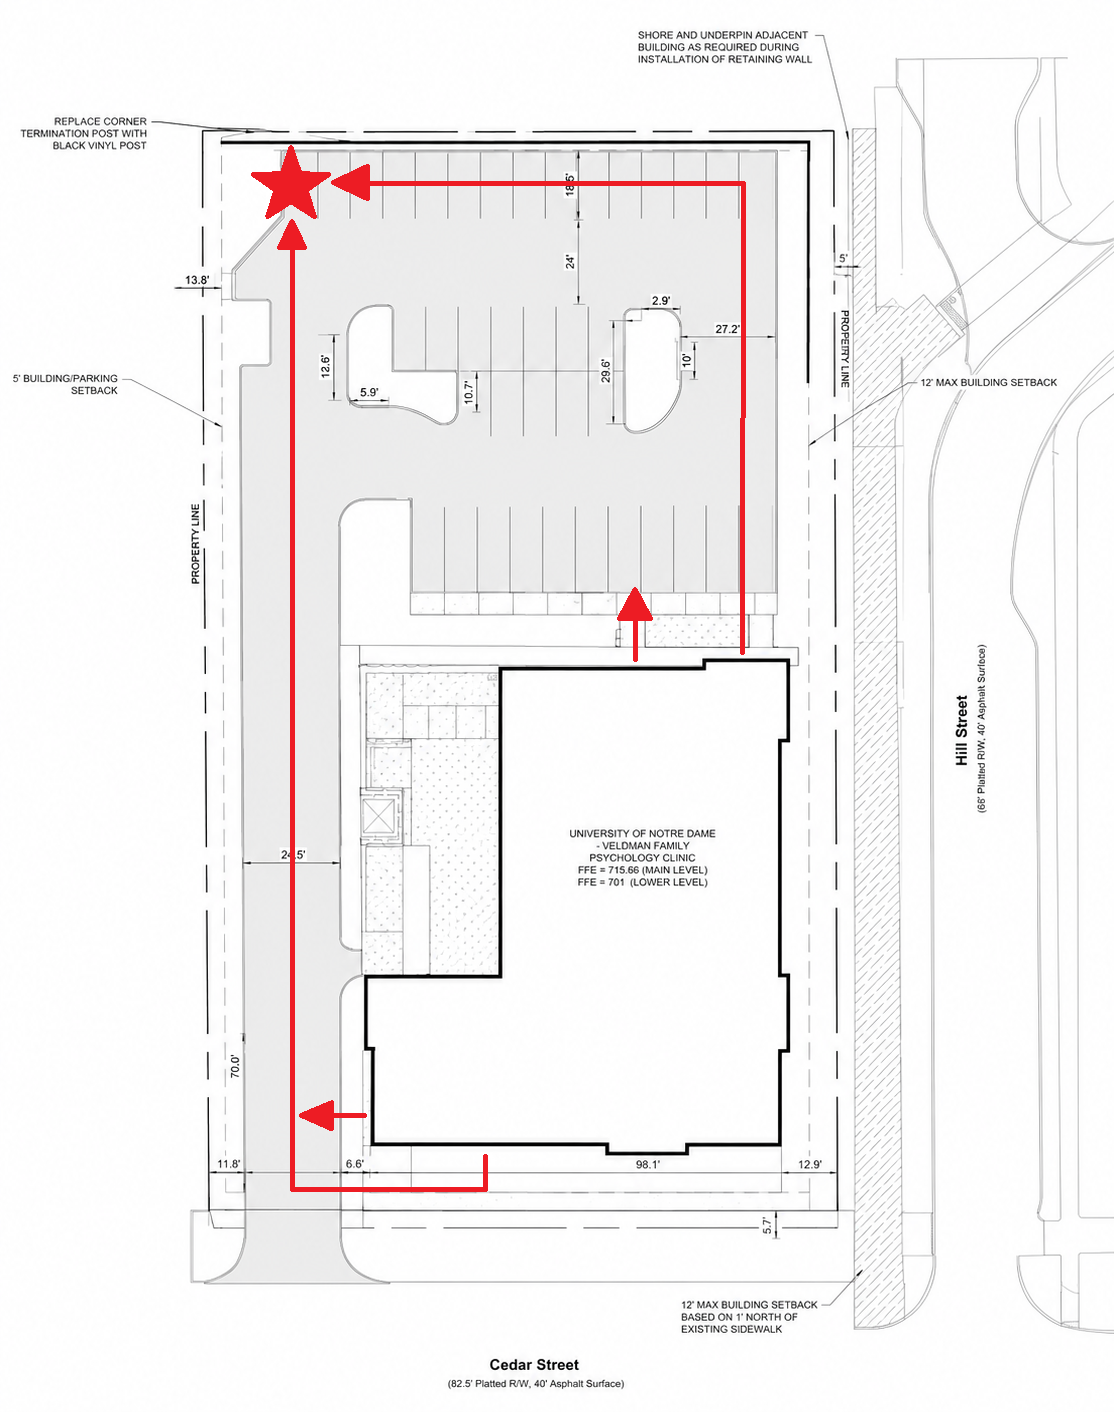
\includegraphics[width=\textwidth]{vfpc_rendezvous.png}
	\caption{VFPC rendezvous location.}
	\label{fig:vfpc-rend}
\end{figure}


\end{document}